% Name: Damped oscillation
% Description: The displacement of an underdamped oscillator, a cosine shrinking inside the exponential envelope ±A e^{-γt}, with its period T marked.
% Tags: damped oscillation, damping, envelope, harmonic oscillator

\usetikzlibrary{arrows.meta}

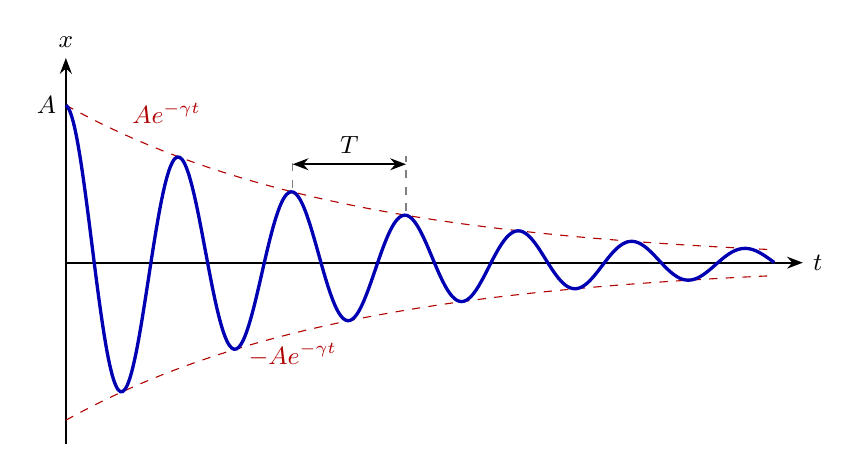
\begin{tikzpicture}[x=0.9cm, >={Stealth[length=2mm]}, every node/.style={font=\small}]
  % x(t) = 2 e^{-0.25 t} cos(2 pi t / 1.6): peaks at t = 0, 1.6, 3.2, ...
  \draw[->, thick] (0,0) -- (10.4,0) node[right] {$t$};
  \draw[->, thick] (0,-2.3) -- (0,2.6) node[above] {$x$};
  \draw[dashed, red!70!black, domain=0:10, samples=60] plot (\x, {2*exp(-0.25*\x)});
  \draw[dashed, red!70!black, domain=0:10, samples=60] plot (\x, {-2*exp(-0.25*\x)});
  \draw[very thick, blue!70!black, domain=0:10, samples=300, smooth] plot (\x, {2*exp(-0.25*\x)*cos(225*\x)});
  \node[left] at (0,2) {$A$};
  \node[above right, red!70!black] at (0.8,1.64) {$Ae^{-\gamma t}$};
  \node[below, red!70!black] at (3.2,-0.9) {$-Ae^{-\gamma t}$};
  \draw[dashed, gray] (3.2,0.95) -- (3.2,1.35) (4.8,0.65) -- (4.8,1.35);
  \draw[<->, thick] (3.2,1.25) -- node[above] {$T$} (4.8,1.25);
\end{tikzpicture}
